\documentclass[9pt]{extarticle} 
\usepackage[utf8]{inputenc}
\usepackage[T1]{fontenc}
\usepackage{lmodern}          %
\usepackage{microtype}       
\usepackage[a4paper,margin=1in]{geometry}
\usepackage{amsmath, amssymb, amsfonts}
\usepackage{mathtools}        % More powerful math extensions
\usepackage{graphicx}
\usepackage{caption}
\usepackage{subcaption}
\usepackage{float}
\usepackage{wrapfig}
\usepackage{tikz}             % Drawing diagrams
\usepackage{booktabs}         % Nicer tabl
\usepackage{array}
\usepackage{multirow}
\usepackage{tabularx}
\usepackage{colortbl}
\usepackage[dvipsnames]{xcolor}
\usepackage[colorlinks=true, linkcolor=blue, citecolor=blue, urlcolor=blue]{hyperref}
\usepackage[nameinlink]{cleveref} % Smarter cross-referencing
\usepackage{enumitem}
\usepackage{fancyhdr}
\usepackage{hyperref}
\newcommand{\notimplies}{%
  \mathrel{{\ooalign{\hidewidth$\not\phantom{=}$\hidewidth\cr$\implies$}}}}
\usetikzlibrary{arrows.meta, positioning}
\pagestyle{fancy}
\fancyhf{}
\lhead{Pricing Options with Mathematical Models}
\rhead{\today}
\cfoot{\thepage}
\newtheorem{definition}{Definition}[section]
\newtheorem{lemma}[definition]{Lemma}
\newtheorem{theorem}[definition]{Theorem}

\usepackage{tikz-cd}
\begin{document}
\begin{titlepage}
    Pricing Options with Mathematical Models
\end{titlepage}
\tableofcontents
\newpage

\section{Stocks, bonds, derivatives}


\subsection{Stocks}

Stocks are issued by firms to finance operations. Essentially 
you purchase shares of ownership of the firm and recieve dividends. Price 
is known today.

\subsection{Bonds}

A bond is an IOU/loan. A contract issued by 
$A$ which if $B$ purchases for $\$x$ (the face value) means $B$ pays 
$A$ $\$x$, in return $A$ 
pays $B$ a total of $\$x+\varepsilon$ over a fixed period of time 
e.g 10 years. The $\varepsilon$ term represents the 
sum of all coupon payments, which are periodic interest payments 
$A$, the issuer, has to pay $B$ in a 
frequency agreed upon in the contract.
The future payoff 
is known at fixed dates, it was pre-determined 
by the contract.


However, in practice when bonds are traded on the market 
things change. Firstly, the future price 
of the bond is unknown, because the price 
represents the value of the bond which depends 
on other factors such as inflation, the interest rate, 
and credit risk of the issuer\footnote{perhaps 
the issuer has suffered irreversible financial loss 
and is now at a high risk of defaulting, this would 
certainly make the bonds less valuable}.
Therefore, a bond may trade for a different 
price than the face value: $\$ p < \$x$, or 
greater than $\$p > \$x$. In each case 
the amount of money we are making changes, and 
this is what bond yield refers to.
\begin{enumerate}[label=(\roman*)]
  \item If $\$p < \$x$, then the bond trades cheap. We purchase 
  it for $\$p$ and we expect to make $\$x + \varepsilon$ the pre-determined
  payoff. Thus, we expect to make $\$x-p+\varepsilon$ profit. If we 
  paid the full face value $\$x$ for the bond, our profit would be 
  $\$x+\varepsilon - x = \$\varepsilon$, i.e we expect to earn just 
  the coupon amount as profit. Thus, if $\$p <\$x$, we say
  the bond \textbf{yield} is higher than the coupon rate.
  \item Similarly, if $\$p > \$x$ then the bond yield is lower than 
  the coupon rate.
\end{enumerate}
The yield is a latent variable, its not observable. We are 
simply saying that the price of the bond differs from face value, so 
we are going to get a different amount of profit. This 
means in reality the 'mean rate of return' per year will be slightly higher than just 
that which was given by the regular cashflow promised by the bond contract. 

Inherently, the higher yield and lower price both represent the same fact: 
the market percieves it to be a risky investment, thus a higher premium (the yield) 
is required for it to be attractive to investors. It is not so simple 
as constantly buying cheap bonds as you will always be taking on risk, 
the efficiency of the market means the risks are already 
priced in: higher yield is merely compensation for bearing higher risk.

\subsection{Derivatives}

A derivative is a contract whose future value is derived from an underlying asset. 
They sell for a price/value/premium. They are traded at either exchanges as standardised 
contracts, there is no credit risk; they can also be traded 
over-the-counter (OTC), institutions find others in a network of individuals and institutions where contracts can 
be more custom made, there is more credit risk. The other side of the deal, the seller if you're a 
buyer and buyer if you're a seller is called your counterparty.

Derivatives are mainly intended to be used to hedge risk. However, their 
uses are multifarious:
\begin{enumerate}
  \item To hedge risk
  \item To leverage convex, non-linear payoffs (in case of options) in speculation
  \item To profit off 'arbitrage' opportunities
  \item To trade one kind of payoff for another (e.g swaps, trading deterministic and stochastic payoffs)
  \item To get around regulations on risk etc.
\end{enumerate}

\subsubsection{Forwards}

Forwards have been around for centuries. A forward is an agreement 
to buy (i.e long) or sell (i.e short) an underlying asset $S$ 
(i) at a predetermined future time $T$ (maturity) and (ii) a predetermined 
future price $F$ (the forward price). The purchase or sale of the underlying to the 
counterparty at maturity 
is \textcolor{red}{obligatory}; there is no option to not purchase or sell. The party which is selling the underlying 
is the seller of the forward, they are the short side; 
the party which buys the forward agrees to buy the underlying, they are the long side. If 
the seller does not own the sufficient amount of underlying they have to short 
sell. 

How is the forward price $F$ determined? It is set so that the contract has 
zero value in the present, meaning if the price right now is $S_0$, then 
$F=S_0f(T,r)$ where $f$ is some function of the risk-free rate; 
this ensures there is no arbitrage opportunity. This means the forward 
has zero value in the present, the value changes later as the underlying fluctuates. 
It also means no cash is paid up front since the value of it at issuance 
is agreed to be zero, its not worth a premia. 

What is the payoff? Delivery of the underlying occurs at maturity $T$. The payoff 
is if you are long $S(T)-F$ and if short $F-S(T)$ where $S(T)$ is the market price of the underlying at maturity. This makes 
forwards a zero-sum game: the gain of one side is the loss of the counterparty. Its a linear payoff also:
\begin{center}
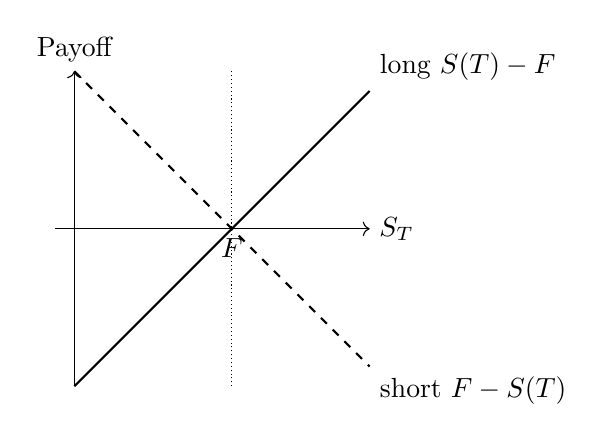
\begin{tikzpicture}[scale=0.5]
  % Axes
  \draw[->] (-0.5,0) -- (7.5,0) node[right] {$S_T$};
  \draw[->] (0,-4) -- (0,4) node[above] {Payoff};

  % Forward price marker
  \def\F{4}
  \draw[densely dotted] (\F,-4) -- (\F,4);
  \node[below] at (\F,0) {$F$};

  % Long forward payoff: S_T - F
  \draw[thick] (0,-\F) -- (\F,0) -- (7.5,3.5) node[above right] {long $S(T)-F$};

  % Short forward payoff: F - S_T
  \draw[thick,dashed] (0,\F) -- (\F,0) -- (7.5,-3.5) node[below right] {short $F-S(T)$};
\end{tikzpicture}
\end{center}
A fundamental use of forwards is and has been to hedge against demand/supply shocks in industry. E.g 
farmers may issue a forward contract which a grain broker buys, wherein both agree that 
the farmer will deliver $X$ amount of grain to the broker at time $T$ for price $F$. Why would the 
broker ever buy the contract? It's just more risk. However, if the broker believes the price of grain at 
$T$ will be greater than $F$, then they would stand to profit from the contract which incentivises them 
to purchase it.


\subsubsection{Swaps}

A swap is an agreement between two parties to exchange 
two \textcolor{red}{sequences} of payments in time. series of forward type payoffs

Example: pension regulations force pension funds to have higher \% investment in fixed-income securities 
as compared to stocks in their portfolio. Pension funds may not want to sell their stocks 
they'd take a loss, so they set up a swap where the stock returns payoffs in time 
are exchanged to a counterparty for fixed-income returns. But the advantage is you don't actually 
sell the stocks, often the holdings are very large so there is an advantage in not selling 
off. When the swap ends operations can begin once more, efficiently. Also there might 
be pressure from firm owners to not sell, potential tax incentives to not sell etc.

An incentive for entering swaps is that by teaming up, akin to the prisoner's dilemma, both 
parties can end up profiting. They aren't zero sum contracts. Swaps exploit comparative advantage (\'a la Ricardo) 
in different markets. For example $A$ might be trusted well in fixed-income markets and not trusted 
in floating, can borrow $5\%$ fixed but only $\text{LIBOR}+0.5\%$ floating. $B$ might be well 
trusted in floating markets but not fixed, can borrow $7\%$ fixed and $\text{LIBOR} +1\%$ floating.
The spread in fixed rates is $2\%$, in floating its $0.5\%$. Then $2/5\% = 0.4 \% > 2/7\%$ so 
$A$ has a comparative advantage in fixed-rate borrowing; $0.5/0.5\%=1\%<1/0.5\% = 2\%$ so 
$B$ has a comparative advantage in floating-rate borrowing. Now $B$ actually benefits 
more from this arrangement since the size of its comparative advantage is smaller. The way 
comparative advantage benefits both is that in negotiation, each party 
is able to buy the good in which the other has a comparative advantage in for a lower 
price than if they were to acquire it themselves, provided the seller (the one 
with the comparative advantage) does not exceed what you could get yourself. A quick diagram:
\begin{center}
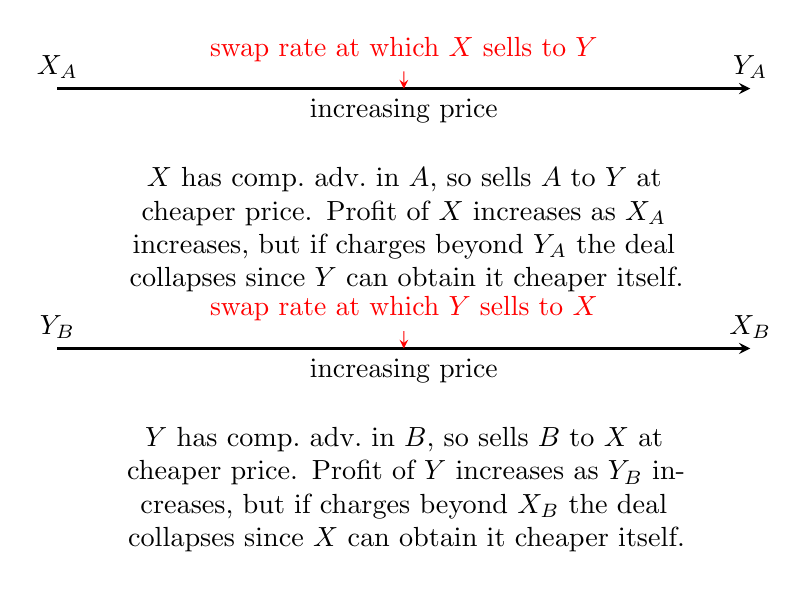
\begin{tikzpicture}[>=stealth,scale=1.1]

% Line 1
\draw[thick,->] (0,0) -- (8,0) node[midway,below] {increasing price};
\node[above] at (0,0) {$£X_A$};
\node[above] at (8,0) {$£Y_A$};
% Swap rate marker
\node[red,above] (swap1) at (4,0.2) {swap rate at which $X$ sells to $Y$};
\draw[red,->] (swap1.south) -- (4,0);
\node[below,text width=8cm,align=center] at (4,-0.8)
  {$X$ has comp.\ adv.\ in $A$, so sells $A$ to $Y$ at cheaper price. 
   Profit of $X$ increases as $£X_A$ increases, but if charges beyond $£Y_A$ the deal collapses since $Y$ can obtain it cheaper 
   itself.};

% Line 2
\draw[thick,->] (0,-3) -- (8,-3) node[midway,below] {increasing price};
\node[above] at (0,-3) {$£Y_B$};
\node[above] at (8,-3) {$£X_B$};
% Swap rate marker
\node[red,above] (swap2) at (4,-2.8) {swap rate at which $Y$ sells to $X$};
\draw[red,->] (swap2.south) -- (4,-3);
\node[below,text width=8cm,align=center] at (4,-3.8)
  {$Y$ has comp.\ adv.\ in $B$, so sells $B$ to $X$ at cheaper price.
   Profit of $Y$ increases as $£Y_B$ increases, but if charges beyond $£X_B$ the deal collapses since $X$ can obtain it cheaper itself.};

\end{tikzpicture}
\end{center}

Imagine wanting a better rate as buying a good, the good is the better rate. This will allow us to map the example with 
rates to the diagram.

Situation: $A$ wants to borrow floating cheaper, $B$ wants to borrow fixed cheaper. So lets suppose $A$ borrows fixed 
at $5\%$ and $B$ borrows floating at $\text{LIBOR} +1\%$ - so $A$ and $B$ have entered into 
exchange with some bondholders or loaners. They then enter into a swap with each other: $A$ 
agrees to pay $B$ $\text{LIBOR}<$A$'s\,\text{lowest possible floating rate} = \text{LIBOR}+0.5\%$; $B$  
agrees to pay $A$ $5.9\% < $B$'s\,\text{lowest possible fixed} = 7\%$. So $A$'s 
position is (i) pays $5\%$ to loaners, (ii) recieves $5.9\%$ fixed from $B$, (iii) 
pays $\text{LIBOR}$ to $B$: effective cost of $\text{LIBOR}-0.9\%<\text{LIBOR}+0.5\%$. 
For $B$ the effective cost of fixed borrow is $6.9\%$. So $A$ saves $1.4\%$ and $B$ $0.1\%$, which 
reflects the greater comparative advantage of $A$ which allows it to extract more value from the 
swap.

\subsubsection{Options}

Options are contracts which give you the right but not the obligation to buy (call) or 
sell (put) an underlying asset at a specified time in the future (maturity). 
European options specify that the option can only be exercised 
at maturity. American options can be exercised at any time before maturity. 
Options can be written on practically \textit{anything} which has a 
numerical value through time:
\begin{enumerate}
  \item Stocks
  \item Indices
  \item Futures
  \item Currencies
  \item Interest rates
  \item Bonds
  \item Credit risk 
  \item Commodities (e.g electricity)
  \item Natural events (weather)
\end{enumerate}
The 
sale of an option is done by the writer/issuer 
of the option contract, this means the seller is 
on the short leg of the call or put; the buyer is the long side. 

Now, the price/value of the 
option through time is the premium. Options have 
a premium at the point of issuance. If exercising 
the option at the present would have been profitable
then its in-the-money; if not its out-the-money. 
If no gain then its at-the-money, although colloquially 
at-the-money options means their strikes are within a $\varepsilon$ range around 
the current price.

We can construct the payoffs mathematically for different positions, depending 
on (i) which contract, i.e put or call and (ii) which side of it we are on, i.e 
long or short:

Long call value/payoff at maturity time $T$ $= \operatorname{max}(S(T)-K,0)=(S(T),K)^+$ where
$S(T)$ is the current price at time $T$ and $K$ is the strike. Means that 
if the option is in-the-money (current $>$ strike) then the payoff is 
$S(T)-K$. If it's at-the-money its just $0$ as $S(T)=K$. If 
current is $<$ strike the option is worthless, the maximum of the two 
is $0$. Since we pay the option premium when we buy the contract at $t$, we lose 
$C(t,K,T)$ which is the premium or value of a call option with strike 
$K$ and maturity $T$ purchased 
at time $t$ today. 
So our profit is just $(S(T),K)^+ - C(t,K,T)$. We have limited downside which is capped 
at the call premium, but unlimited upside. The reason for the payoff being 
defined that way is due to arbitrage; if we can buy the underlying for $S(T)\leq K$ 
then there is no incentive to pay the premium, so the value of the contract is worthless. 
On the other hand, if the price is far above the strike then there is an incentive to 
buy the contract as there is an arbitrage: you can buy at $K$ then sell at 
$S(T)$ and make a profit. That is the value of the contract, how much you could make 
by exercising it; thus its premium/value 
must be $S(T)-K$ when the underlying is $>$ strike.

Suppose we are on the long side of a call. The payoff and profit 
graphs are as below. 

We need to make the premium back to break even, so the breakeven price 
is the call premium $+ K$, because the option is only worth something 
once its ITM, so after breaching the strike we need a movement of $S(T)$ upwards 
as large as the premium.


On the short side, everything is flipped. The payoff at maturity $T$ is 
$-\operatorname{max}(S(T)-K,0)$, the profit is  $-((S(T),K)^+ - C(t,K,T))= 
 C(t,K,T) -  (S(T),K)^+ $. The upside is limited at the premium, the downside is 
unlimited. The breakeven price is the same as the long side's: call premium $+ K$


Long put value/payoff at maturity time $T$ $= \operatorname{max}(K-S(T),0)=(K-S(T),0)^+$. Puts 
gain in value in an inverse relation to calls. Puts are ITM when 
current price is $<$ strike because this means we can buy the asset, then exercise put and sell them 
at a higher price. By the same arbitrage arguments when the current is $\geq$ strike then 
the contract is worthless. The profit for the long side is the 
payoff of the put - the premium, the short side's is the premium - the payoff of the put. The short 
side of a put is less dangerous than that of a call since an asset's price is limited from below by $0$ - there 
aren't negative prices. But in practice the risk is about the same for stable, high value assets such 
as the FTSE since a $5000$ move up or down is about equally likely, and an unlimited rise is just 
nonsense but still theoretically possible.


Heuristic: short side's payoff and profit is $-$ of long side's.
Heuristic: payoff graph of short side is the long side's reflected along $x$-axis; payoff of put 
is the payoff of call reflected across $x=\text{break even price}$. 


Option payoffs can be found almost everywhere there is a non-linear payoff with fixed downside. An example 
would be equity linked bank deposits where someone invests a fixed amount of money, 
and if an index stays below a price in the future (the strike) then you gain no money on top 
of your investment; if it does exceed the strike then you get a linear transformation of the 
return on the index applied to your investment. Thus the payoff is that of a bond (you invested a fixed amount 
and recieved a fixed amount back) $+$ a linear 
transformation of a call option on the index. Since the payoffs can be mapped 
to these known financial instruments the bank can price the 
contract in a way that on average benefits them, 
using the market data. Calls are thus mostly 
speculative, in a sense they're hedges against losing 
during the rise of the underlying; puts are hedges against losing during the downturn of the 
underlying.

Combining options: bull spreads are constructed by going long on a strike 
less than the current price and short (selling) on a strike greater than the 
current price. This holds for both calls and puts. The converse is true for 
bear spreads: you go long on a strike greater than the current price and 
short on a strike less than the current price. So you're either 
believing the market's going up (bull spread) or down (bear spread)
but you want to hedge your position so also sell an option (in case 
of bull) or buy (in case of bear) at a strike that is further 
along your expectation because you believe from that point on its unlikely
to persist in the same direction as the long side was based on, and is more likely 
to reverse (thus going the opposite leg would protect you against losing what 
you made on the initial leg). So bull/bear spreads are based on a 
sentiment on which way the market is going: directional. There are other 
combinations however which focus on the total range of price movement in a period, regardless 
of direction; they are volatility based. You can either be short (lose from; fragile) or 
long (gain from; antifragile) volatility. Butterfly spreads are short volatility: 
you profit from the underlying staying within a small range of values (hurt by large volatility); 
constructed by going long on strikes set at different prices in the future - the absolute 
difference of these strikes is the range in which you think the price stays, to hedge against you 
being wrong you sell two options with strikes roughly in the middle of the range (although it could 
be anywhere depending on your analysis of the market), the premium of which will mean you don't get annihilated 
by an adverse movement. Straddles are skewed in the opposite direction to butterfly spreads, since they take 
the opposite position on volatility; we lose if the volatility stays low but benefit when it breaks the bound. In general, the main heuristic is \textcolor{red}{Go long on your 
expectation (e.g long call, long put, combination of long calls and/or puts)}, \textcolor{blue}{hedge (make sure the premia don't add up to annihilate you) 
by going short on the opposite}. It's irrelevant whether you use puts or calls, you can 
create the payoffs with either; calls are more convenient.

The tables for the payoffs of these different combinations could be  and they are trivial to 
calculate, it's just case work; but they are 
a practioner thing, in this course we are not really going to use them so its best to 
save that for the document in the grand codex later on.

The above combinations are examples of statically hedged positions since we enter at the start 
and don't change them. 


The arbitrary payoff of an option (note this is payoff, not profit; its not including the premium), $f$ at some price of the underlying $s$ is given by 

$$f(s) = f(0) + f'(0)s + \int_{0}^{\infty} f''(K) \operatorname{max}(s-K,0)\,dK$$
where $K$ represents the strike prices, which are assumed to be infinite. This is the Breeden-Litztenberger 
formula. By doing 
integration by parts on the integral the entire formula follows. The thing to remember here is that 
this is \textit{replicating} the payoff of an option; let's go through why each of the terms is necessary in this replication:
\begin{enumerate}
  \item $f(0)$ - represents the cash value of the contract at $s=0$; e.g for a short call it is the premium, for long call it would be $-$premium 
  \item $f'(0)s$ - linear exposure to the underlying by owning it. This is needed because at maturity the option payoff 
  will be exactly what we saw in the diagram, it will have a kink at the break-even price which cannot be represented by a differentiable function.
  \item $\int_{0}^{\infty} f''(K) \operatorname{max}(s-K,0)\,dK$ - this is the source of non-linearity in the option payoff. The payoffs of 
  vanilla calls are the basis vectors in the function space of payoff functions on $s$, we can represent an arbitrary non-linearity in the 
  payoff in terms of this. The coefficients $f''(K)$ in the integral tell you how much weight you need to assign 
  a specific call in your basket/portfolio of calls to replicate the payoff. 
\end{enumerate}
The point is that that 
any option payoff can be replicated statically using 
only cash, underlying, a basket of vanilla options across strikes. In fact 
this generalises to the payoff of any elementary security.
This is what makes the volatility surface valuable, because using the principle above, from the 
surface you can derive the risk-neutral
probability density of the underlying price at (uses stochastic calculus to model how 
the asset price varies). This 
distribution allows you to then price any payoff function on 
the underlying.

\section{Pricing deterministic payoffs}


The point of understanding how deterministic payoff assets 
are priced, such as bonds, is that they are used in the pricing of 
options later on. Often deterministic payoff pricing is called 
'present value calculations'.
\subsection{Basics of interest payment}
Quick note on interest rate conventions:
\begin{enumerate}[label=(\roman*)]
  \item Simple interest: after $T$ years, future value of \$1 in a bank account is 
  $1+Tr$
  \item Interest compounded once a year: $(1+r)^T$
  \item Interest compounded $n$ times a year: after $m$ compounding periods the 
  future value is $(1+r/n)^m$. This splits up the payoff into the compounding periods, 
  $m$ can be as large as we want. Suppose $n=4$ so a quarterly compound, but we choose a 
  overall time frame of 10 years - then there are $m=10\cdot 4=40$ compounding 
  periods. So $m=nT$ where $T$ is the number of years considered in time frame. Note that the reason $n$ divides $r$ here is that $r$ is the nominal 
  annual rate; in the case of compounded once a year this is just the same as what we 
  get, but with $n$ times a year in each compounding interval (quarter in our example) 
  we only get $1+r/n$ growth not $1+r$.
\end{enumerate}
In practice, almost everyone uses (iii). With interest compounded $n$ times a year, 
since the actual annual return is latent as we are not getting annual payoff but rather 
$n$-periodly, we have to try and approximate it. This is the concept of 
the \textit{effective annual interest rate} $r'$ which is given by 
interest compounded $n$ times a year after $n$ compounding intervals (a year)
$$1+r' = (1+r/n)^n $$
E.g quarterly compounding at nominal annual rate of $r=8\%$ gives 
$(1+0.08/4)^4 = 1.0824 = 1+0.0824$ and so the effective annual rate 
is $r'=8.24\%$. In essence, we check the return after a year under the scheme of 
compounding $n$ times a year. You can only derive this from 
a given nominal rate, or vice versa.


Note also that if we take $n\to \infty$ 
we begin to approximate a continuous, perpetual compounding. Because $356/n$ as 
$n\to \infty$ will give us infinitesimally small compounding intervals which 
approximates instantaneous, continuous compounding at every moment. Mathematically, 
when we do this 
$$\lim_{n\to \infty} (1+r/n)^m = \lim_{n\to \infty} (1+r/n)^{nT} = e^{rT}$$
so the payoff of interest compounded continuously over a time frame of $T$ 
years is $e^{rT}$. The annual rate when compounded continuously gives 
lowest present value.


\subsection{Price as present value}

The principle which underlies replication and the essence of option/random 
payoff pricing later in the course is the \textcolor{red}{law of one price: if two 
series of payoffs, i.e cash flows deliver the same payments in the future, they have the same price/value 
today.} This is based on no-arbitrage principles, because if it didn't hold you 
would have an arbitrage opportunity where you buy the cheap one and sell 
the expensive one.
Thus, we can define price as: if one can \textit{guarantee} having $\$X(T)$ at time $T$ by 
investing $\$X(0)$ today, then today's price/value of $X(T)$ is $X(0)$. The term 
$X(0)$ which becomes the current price is the present value PV$(X(T)$) when we consider 
deterministic $X(T)$.

Therefore, suppose we invest $X(0)$ at compounded interest rate of $r/n$ over $m$ periods then 
$$X(0)(1+r/n)^m = X(T) $$
for some $X(T)$; so we can guarantee $X(T)$ by investing $X(0)$ today, 
so the current price of the asset has to be 
$$ X(0) = X(T)/(1+r/n)^m$$
In other words, we apply a discount factor of $1/(1+r/n)^m = e^{-rT}$ to the 
future price $X(T)$, for appropriate parameters $m,T$.

Now, suppose instead we have a sequence of payoffs 
$X(0),X(1),\ldots,X(m)$ paid at the end 
of each compounding interval. Recall then that if we can guarantee 
$X(T)$ by investing $X(0)$ today the current price, the present value is 
$$\frac{X(T)}{(1+r/n)^m} $$
Since the $X(i)$ are compounding interval payoffs, clearly they follow the rule 
$X(1)=X(0)(1+r/n)^1, X(2)=X(0)(1+r/n)^2,\ldots$. We can guarantee $X(1)$ 
by investing $X(0)$ today, that adds value to PV; we can also guarantee 
$X(2)$ today on top of that $X(1)$, that adds further value; and so on until we get to $X(m)$. So the present 
value is the sum of the present values when we 
consider all of the $X(i)$ up to $X(m)$
\begin{align}
  PV = \sum_{i=1}^m \frac{X(i)}{(1+r/n)^i}  
\end{align}
when $X(i)$ is constant it becomes a geometric series. So the present value is the sum of 
the discounted cash flows/payoffs. Heuristic for discounting: the value now is the 
value in the future, divided by the steps that take us to it - which we won't have received yet.

\textcolor{blue}{The asset here does not have to be an interest receiving payoff, it can 
be any deterministic payoff. The 
point is that we are using the law of one price to 
price $X(T)$: if we know for certain that an asset $X$ will deliver 
$X(T)$ at time $T$ (certainty = deterministic) then we could simply invest 
a certain amount 
$X(0)$ at the risk free rate today under compounding and it 
will deliver $X(T)$ at time $T$. By the law of one price since both 
deliver the same deterministic payoff, both have the same present value. Thus, 
the present value of the asset $X$ can be obtained by the convenient 
PV formula.}

If we take a loan, ie we are on the opposite side of the deterministic payoff, 
then the PV is the loan amount and so you can rearrange to find out the 
fixed amount $X$ you should be paying every compound period.

\subsection{Bonds}

Suppose a bond pays a face value $V$ at maturity $T=m$ periods 
and $n$ identical coupons per year of value $C/n$ (these are the coupons paid per 
compounding interval) and the bond price today is $P$. In essence we have a 
sequence of payoffs $B(1),\ldots, B(m)$ each giving $C/n$. We know that since 
we can guarantee the amounts $B(i)$ by 'investing' some amount $\Omega$ today, by the law of one price the 
present value of each of these $B(i)$ must be $B(i)$ discounted by 
the rate that would get you there from the amount $\Omega$ invested today. Thus the 
total present value from the coupons is 
$$ \sum_{i=1}^m \frac{C/n}{(1+r/n)^i}$$ 
However, there is also the face value $V$ which must be paid back at time $m$ - we need to account for this 
in the present value too. Thus, in actuality, the 
payoff at time $m$ is $V+C/n$ not merely $C/n$; the present value of this is again $V+C/n$ discounted by 
the rate that takes you there from the amount $\Omega$ invested today. This means the PV of this bond is 
\begin{align}
  PV_{\text{bond}} = \frac{V+C/n}{(1+r/n)^m} + \sum_{i=1}^{m-1} \frac{C/n}{(1+r/n)^i}\label{bondprice}
\end{align}
and this is the amount $\Omega$ that we would need to 'invest' today to get the bond payoff. Think about it - if we multiply 
$PV_{\text{bond}}$ by $(1+r/n)^m$ we get $V+\sum_{i=1}^{m}\frac{C}{n}(1+r/n)^{m-i}$ which is exactly the payoff of the bond: face value 
plus the coupons, inflated by the amount of interest (yield) each earned.
\textcolor{red}{The rate $r$ that satisfies this equation is the bond yield. It is interest which accrues on the coupons: each coupon 
earns the yield rate of interest $/n$ over each compounding period, the earlier a coupon is distributed the more 
compounding periods it has to earn interest and thus it's value at the end is greater. 
The yield is a latent variable that must be inferred 
from the market, like implied volatility.} The price equation 
\eqref{bondprice} is non-linear so must be solved numerically.

We can infer from \eqref{bondprice} that the larger the coupon the higher the price of the bond. This is 
somewhat of a reality check for the model 
as it's obvious that if we are recieving more per period then it will make the contract more valuable.

Another thing we can infer is that if the bond price $=$ the face value, ie the bond trades at par, 
then the coupon rate (the fixed \% of the face value paid per period) must equal the yield.

\textcolor{red}{Spot rate is the yield of a zero-coupon bond.}

In practice how might we go about finding the price, so as to be able to then find the yield of some bond? Again, we use 
the law of one price through replication. It turns out if we know the price of a zero-coupon bond and a coupon-bond we can 
replicate the payoff of another zero-coupon bond with different maturity using combination of long/short positions; the cost of the 
replicating payoff defines the price of the new bond and the gain from the replicating payoff defines the future guaranteed payoff of the new 
bond. \textbf{Add the specific example/numbers at some future point.} Then by the law of one price the yield is just the $r$ s.t $(1+r)$ times price $=$ future value. If we priced it differently then 
we would have that the price of the new bond is expensive then there would be an arbitrage 
as you can construct a long/short payoff which replicates the new bond payoff exactly for cheaper; then you short sell 
the expensive, this means you borrow the bond from someone and immediately sell it for the inflated price earning $X$; if we wait until 
maturity to exit our short position, the bond matures/expires into its cash payoff so you have to 
pay the bond payoff to the one you borrowed it from since they would have had that if 
they kept the bond\footnote{For assets with no expiry like stocks you have to return the number of shares you borrowed, which means buying back. Here there is now 
risk involved since you cannot deterministically replicate the stock payoff using some replication, so we don't know if the cancellation 
of long/short repayment will be perfect, it ceases to be a perfectly risk-free arbitrage.}; since the replication you bought for cheaper, incurring cost $X-\delta$, 
gives the exact same payoff you just use that to pay back the guy you borrowed it from. Thus you net $X-(X-\delta)=\delta$ (ofc the 
margin cost is not included here).


We can also replicate the payoff of a zero-coupon bond which matures at period $j$ 
using a zero-coupon bond of shorter maturity at period $i<j$; this is given by 

$$(1+r_j/n)^j = (1+r_i/n)^i(1+f_{i,j}/n)^{j-i} $$
where $r_k$ is the annualised yield on the zero-coupon bonds, there are $n$ compounding periods in a year, 
and the rate $f_{i,j}$ which solves this is called the forward rate. We are replicating 
the payoff at $j$-th period by using an $i$-period bond and then trying to find the rate over the $i-j$ gap period 
which gets us to the $j$ payoff; the $=$ is given by the law of one price. So this is another no-arbitrage relationship. Again, this gives arbitrage opportunities
where you can speculate on whether the forward rate, i.e the rate between the $i$-th and $j$-th periods you would 
need to invest your $i$-period bond in to get the $j$-period payoff, is over or undervalued. Suppose the $i$-period bond 
gives a payoff of $X$ at maturity, then the $j$-period payoff is given by $X/(1+f'_{i,j})$ where $f'$ is our 
estimate of the forward rate. Then we buy a $j$ and short $i$ in proportion s.t we 
incur zero cost. After $i$ period we close the short and pay back the bond payoff to the loaner, 
if $f'=f$ i.e no-arbitrage then the payoff we'd get on the long side would be identical to what 
we lost on the short side; however if we're right and $f'<f$ then what we receive on the long side 
will be guaranteed to exceed what we lose on the short side.

\newpage
\section{No-arbitrage pricing relations}

\subsection{Pricing forwards}
\textcolor{red}{THIS SECTION NEEDS TO BE REVIEWED AGAIN: BASED ON THE MISUNDERSTANDING OF THE LAW OF ONE PRICE 
I STATED THAT THE REPLICATION IS BEING DONE SO THAT THE VALUE OF THE REPLICATION IS 0 AT INCEPTION, I.e MATCHING 
THE FORWARD'S VALUE AT INCEPTION. THIS IS WRONG. THE FORWARD's VALUE IS 0 UP UNTIL MATURITY, AND THE 
LAW OF ONE PRICE DEMANDS THAT AN ASSET AND ITS REPLICATION, i.e TWO SERIES OF PAYOFFS, 
MUST AGREE IN THEIR PAYOFFS AT EACH AND EVERY TIME STEP OF THEIR DURATION. ONLY THEN CAN THE LAW BE APPLIED TO DEDUCE THEIR PRICES TODAY 
ARE IDENTICAL.}


Consider a forward on underlying $S$ entered at $t$ with payoff 
at maturity $T$. The payoff is $F(T)=\pm (S(T)-F(t))$ ($+$ in long/buyer of 
forward, $-$ in short/seller/issuer of forward) where $F(t)$ is 
the forward price decided at $t$. The forward price is kind of like a premium 
because it is deducted from the winnings of a long position on forwards 
and given to the short side of the contract.

The pricing goal is to ensure that the contract \textcolor{red}{value} is worth $0$ 
at time $t$, which means finding a suitable $F(t)$ such that at $t$ the payoff is $0$. It's a 
bit confusing but the value of the contract is the payoff, and that's given by 
$F(T)=S(T)-F(t)$. At $t$ this value is $S(t)-F(t)$. So 
we want to find a $F(t)$ which makes this 0 - this is the pricing problem.


We proceed using law of one price and no-arbitrage. We invest $\$1$ at the 
risk-free rate at time $t$ and it results in payoff $B(t,T)$ at time $T$. This 
can be whatever kind of compounding we want. The point is we \textcolor{blue}{claim:
the $F(t)$ that solves the pricing problem is} 
\begin{align}\label{forwardp}
  \textcolor{blue}{F(t) = B(t,T)S(t)} 
\end{align}
that is, there is no arbitrage $\iff$ \eqref{forwardp} holds.

Motivation: let's recall that a forward contract stipulates that the long side must 
buy the underlying at a future time and an agreed upon future price - the forward price, and the short side must sell it at that 
price. We want to replicate the payoff of the forward and then we will get our answer. We need to replicate 
having $S(T)$ in the bank with a liability $F(t)$ (i.e payoff/value of $S(T)-F(t)$) such that the cost/value of the replication is 
0 at inception. This mimics the forward's payoff and its 0 cost at inception:
\begin{enumerate}
  \item Borrow underlying at the risk-free rate today: gain $S(t)$ immediately, loan amounts to $S(t)B(t,T)$ altogether over the contract duration 
  \item Purchase the underlying immediately at the current price $S(t)$ with that money: now we own underlying
  \item Note how the cost at inception is 0: Gained loan money worth $S(t)$, lost $S(t)$ on purchasing asset: thus cost of portfolio at inception is $S(t)-S(t)=0$
  \item At maturity the underlying we hold is now worth $S(T)$: we have $S(T)$ worth of money in our bank account 
  \item However, we now owe $S(t)B(t,T)$ from the loan to the loaner
  \item Thus our payoff at maturity is $S(T)-S(t)B(t,T)$
  \item By law of one price since this replication has an identical payoff to the forward and satisfies the condition of 0 cost at inception, we obtain 
  $$S(T)-F(t) = S(T)-S(t)B(t,T)\implies F(t)= S(t)B(t,T) $$
  \item Thus the forward price is indeed given by \eqref{forwardp}.
\end{enumerate} 


Proof: to verify that this enforces no-arbitrage we consider $F(t)\neq B(t,T)S(t)$, viz. $F(t)>B(t,T)S(t)$ and $F(t) < B(t,T)S(t)$.
\begin{enumerate}
  \item $F(t)>B(t,T)S(t)$: at inception borrow $S(t)$ at risk-free rate and purchase underlying at $S(t)$, short the forward (sell). At maturity 
  we receive the 'premium' of $F(t)>B(t,T)S(t)$ which exceeds our liability from repaying the loan: $B(t,T)S(t)$. Owning the underlying 
  means the $S(T)$ gained from it and lost from the forward payment cancel out. We thus make risk-free profit of $F(t)-B(t,T)S(t)>0$
  \item $F(t)<B(t,T)S(t)$: at inception we invest\footnote{I.e we earn interest on it.} $S(t)$ at risk-free rate and short a unit of underlying, we also 
  buy the forward. At maturity since we earned $B(t,T)S(t)>F(t)$ over the period of the contract we have more than enough to 
  pay the forward 'premium' of $F(t)$. The $S(T)$'s gained and lost from the forward and short respectively cancel out. We make risk free profit 
  of $B(t,T)S(t)-F(t)>0$. 
\end{enumerate}

All of the above can be souped up by introducing dividents paid on the underlying. Then \textcolor{red}{$F(t)=B(t,T)(S(t)-D(t))$} where 
the present value of the dividends is $D(t)=D/(1+r/n)^m$. For continuous compounding we just have forward price with underlying paying dividends is
$F(t) = B(t,T)e^{-q(T-t)}S(t)$ where $q$ is the rate per infinitesimally small period of time. Moreover, using the 
framework in the proof depending on whether $F(t)$ is $<$ or $>$ the no-arbitrage price you can follow the same process 
(long, short, invest/borrow etc) and get an arbitrage.


\subsection{Pricing futures}

\textcolor{blue}{Motivation, basic mechanics}: why do we bother with futures? It stems from forwards. Forwards are impractical as to determine the amount needed 
to be paid at maturity $T$, i.e $F(T)$, you need to know what $S(t)$ was at $t$ when you entered the contract - as per \eqref{forwardp}. Moreover, 
there is a credit risk because the other party could go bankrupt and you would have no protection against it. So we create contracts called 
futures, which are ways to implement forwards without the above two difficults: we trade the future against an exchange which is assumed to 
have no credit risk (obviously fanciful but the likelihood is what matters). Moreover, the payoff from the position is settled every day 
in your \textcolor{red}{margin account} with the exchange - this is called marked-to-market. So if you made a gain that day you get the gain in your account, if you lost 
you get the loss deducted. Note that with the margin account you have to deposit a certain \% of the total contract value 
at the start to show you could weather losses - this is the \textcolor{red}{initial margin}; once the contract is entered you have to have a certain amount in it 
every day to remain solvent, this amount is called the \textcolor{red}{maintenance margin}. The maintenance margin is always less than 
the initial margin. 

Each day after the marked-to-market process is settled your margin account is reviewed by the exchange to see 
if you meet the margin requirements: if you drop below maintenance margin you're issued a \textcolor{red}{margin call}, which means 
you have to deposit funds into the margin account such that you get back up to the \textit{initial margin} amount, not just 
back to maintenance. If you fail to do this within the deadline your position is liquidated meaning your positions are closed 
and whatever is gained is used to cover the amount your account is below the maintenance margin and top it up to the initial margin level. In the worst case scenario, since 
we're dealing with leverage, 
we may end up losing so much that our entire margin account gets wiped out. If thats the case we enter negative balance - we've lost more money in the trade (leverage means 
you've borrowed the leveraged amount that gives you access to more exposure of the asset, from the exchange) than we could even afford to. 
We now owe the exchange the negative balance as well because its their money we have lost. 

So the margin account is a stopgap, if losses during liquidation
are within the range such that closing the position leaves you with non-negative balance, you've just lost that amount and nothing owed. We're operating 
a bit above the wave of the loaned amount via leverage. But if we lose more than the balance we've fallen under and must pay the exchange.
This eliminates credit risk on behalf of 
the exchange; they don't let losses spiral, you're automatically closed out. So we've resolved both issues with forwards: impracticality and credit risk.


\textcolor{red}{Pricing futures:} the obvious idea is to replicate the futures payoff using forward contracts then use the law of one price. Now, the futures payoff every 'day' 
is just the realised profit of the forward its based on. So the payoff (profit/loss) is 

\begin{align}
  \text{Future contract payoff} = (F(t+1) - F(t)) + (F(t+2)-F(t+1))+ \cdots + (F(T)-F(T-1)) = F(T) - F(t)
\end{align}

However, the future pays throughout the contract on each day via marked-to-market, whereas the forward pays all at once at the end. Now the \textcolor{red}{the law of one 
price, however, demands something specific: two series of payoffs with the same payoffs at the same \textit{times} must have the same price today} note that 
the end sum might be equal but if the \textbf{paths to get there} do not agree in terms of the payoff at each time step, then we cannot use the law. So \textbf{we must 
make the payoffs at each time step agree}. 

To do this \textcolor{blue}{we can use a trick.} We want the payoffs at each time step to agree. Forwards have 0 payoff at any time before the 
maturity, by design. So our replication must agree with that: just to be clear 
we are trying to replicate a forward's payoff using futures. Its actually quite simple. 
\begin{enumerate}
  \item We begin by buying at $t=0$, $e^{-r(T-1)}$ worth of a future. Note that $F(t)$ here will refer to the price of the future.
  \item At $t=1$ we increase it to $e^{-r(T-2)}$.
  \item At $t=i$ we buy $e^{-r(T-(i+1))}$ worth of a future.
  \item Now, at each time step when we make a profit/loss from the future, namely the difference 
  $F(i+1)-F(i)$ multiplied by the amount we own $e^{-r(T-(i+1))}$, we want to make sure that our payoff at this time 
  us 0. Because remember, we need our replication to agree in payoff with the forward's payoff at each time step.
  \item How do we make sure of this? Well, when we gain money from the future i.e $F(i+1)-F(i)>0$, we 
  spend that money on a bond equal in value that matures at $T$. So we're cash neutral. If we lose money from 
  the future i.e $F(i+1)-F(i)<0$ then we sell a bond for value equal to how much we lost. So we're cash neutral. That it is possible to find 
  a counterparty to these at these specific values is an assumption made: we go to the money market and there is always liquidity for whichever
  bond we want to buy/sell.
  \item Obviously, if we bought the bond for $e^{-r(T-i)}(F(i+1)-F(i))$ then at maturity, since 
  we earn interest from our counterparty in the bond sale, the amount we will recieve will just 
  be $e^{r(T-i)}(e^{-r(T-i)}(F(i+1)-F(i)))=F(i+1)-F(i)$. If we sold the bond for that much then the amount 
  we would have paid off to the counterparty at maturity would be the same. Since the directionality of losing money from 
  the future and gaining money is determined precisely\footnote{This works beacuse if we make a loss automatically the term in parentheses becomes negative and thus 
the $e$ term becomes negative representing how we lose money from the fact we have to pay the bond off. If it's 
positive we earn the money from the bond since we bought it.} by the sign of $F(i+1)-F(i)$, we \textbf{now know then that 
the value of the futures profit/loss realised in marked-to-market at $t=i$ will end up at $F(i+1)-F(i)$ at maturity}.
\item This means at maturity our replication will have accumulated the payoffs\footnote{We did this legally, we agreed with forward 
payoff at each time step from $0$ to $T-1$. What remains is maturity.}

\begin{align}
  \sum_{i=0}^{i-1} (F(i+1)- F(i)) = F(T) - F(0) = S(T) - F(0)
\end{align}
\item If rates are deterministic then the payoff of the future at maturity will be equal to the payoff of the forward corresponding to it. Thus 
we have guaranteed agreement in the payoffs of the future and forward at every time step including maturity. 
\item By the law of one price, since we replicated the payoff of a forward entered into at time $t=0$ at each time step, we must have that the future 
price today, namely $F(0)$, and the forward price today are identical. 
\end{enumerate}

Since rates are stochastic in reality step 8 does not hold which leads to differences in prices between forwards and futures. I don't need 
to go into this right now, but in the future this seems like an area that a lot of practioners must be working on. 

\subsection{Pricing swaps}

For simplicity we are only covering interest rate swaps pricing. If we are the long side on an interest rate swap we are receiving the floating rate 
$L$ and paying the fixed rate $R$ at time $T_i$, so our payoff/position at point 
$i$ is, assuming the time between consecutive time points $T_i$ is fixed at $\Delta T$ 
 
\begin{align}\label{swp}
  C_i = \Delta T (L(T_{i-1},T_i) - R)
\end{align}
where $L$ refers to the LIBOR rate
\begin{align}\label{lr}
L(T_{i-1}, T_i) = \frac{1-P(T_{i-1}, T_i)}{\Delta T P(T_{i-1},T_i)}
\end{align}
where $P(T_{i-1},T_i)$ refers to the price at time $T_{i-1}$ of a zero-coupon (default-free) bond that matures at $T_i$ paying 
$\$1$ at maturity (remember zero-coupon means only the face value is paid off at the end). It's not particularly 
important why LIBOR is defined as this for our purposes.


This isn't too difficult to grasp. It's just profit or loss, if the LIBOR rate is paying us more than 
the fixed rate we win, if  not we lose. The gain/loss is realised after one time step wherein the LIBOR 
rate actually moves.

If we plug in \eqref{lr} into \eqref{swp} and rearrange, we can get the swap price purely in terms of the zero-coupon bond, 
the fixed rate and time:

\begin{align}\label{swpprice}
  C_i = \frac{1}{P(T_{i-1},T_i)} - (1+R\Delta T) 
\end{align}

So we have replicated the payoff of the swap using \eqref{swpprice}, but there are two different pieces in it we have used 
which correspond to different objects. The first term involves using bonds the second is a fixed amount invested at the 
fixed rate. 
\begin{enumerate}
  \item Recall that the payoff at time $T_i$ from a single swap period is 
  \[
    C_i = \frac{1}{P(T_{i-1},T_i)} - (1+R\Delta T).
  \]
  This payoff occurs at $T_{0\leq i\leq n}$ and must be replicated today at $t < T_0$.
  
  \item Start with the floating leg payoff $\tfrac{1}{P(T_{i-1},T_i)}$ at $T_i$.  
  To replicate this, at time $t$ we purchase $P(t,T_{i-1})$ worth of a zero-coupon bond maturing at $T_{i-1}$.
  
  \item At time $T_{i-1}$ this bond pays $1$. We immediately use that earning to buy exactly $\tfrac{1}{P(T_{i-1},T_i)}$ zero-coupon bonds maturing at $T_i$.
  
  \item We then receive precisely $\tfrac{1}{P(T_{i-1},T_i)}$ at $T_i$ thus 
  agreeing with the first term in \eqref{swpprice}.  
  
  \item Next, consider the fixed leg payoff of $(1+R\Delta T)$ at $T_i$.  
  This is just a deterministic payoff. Since we owe this amount at time $T_i$ all 
  we have to do is invest this amount into a zero-coupon bond that matures and pays at $T_i$ 
  $P(t,T_{i})$ bond, meaning we would need to pay $P(t,T_i)(1+R\Delta T)$ at $t$; since it will return $1$ at $T_{i}$ we obtain $1+R\Delta T$, the second term in \eqref{swpprice}.
  \item Now using the replications in steps 4 and 5 we have replicated the payoff of the swap at each time step $i$. 
  \item Using the law of one price applied to steps 4 and 5, we know then that the value of the payoff $C_i$ at time $t$, i.e today, is 
  \[
    C_i(t) = P(t,T_{i-1}) - (1+R\Delta T) P(t,T_i).
  \]
  Because after inception the zero-coupon pays nothing until the time $T_i$ - exactly what the payment at the time $T_i$ is doing. Therefore our 
  replications price at $t$, namely $(1+R\Delta T)P(t,T_i)$ must be the price/value at $t$ of the payment at $T_i$. This is how we get the present value. 
  Similarly, we do it for the $1/P(t,T_{i-1})$ term. 
  \item Summing over all periods $i=1,\dots,n$, the total replication price at time $t$ is then 
  \[
    S(t) = \sum_{i=1}^n C_i(t).
  \]
  This gives us the price today of the replication.
  \item By the law of one price, and using step 6 - the fact that the payoff agrees with the swap's all throughout, 
  the price $S(t)$ we obtained by replication must equal the actual price of the interest rate swap at time $t$.
\end{enumerate}

\textcolor{blue}{So law of one price application seems to follow: create replication, check payoff is equal all throughout $t=1,\ldots,n$, then the payoff at start i.e the present value / price 
today i.e at $t=0$ is the same as the replication's.}

\subsection{Some inequalities and relations for options}

The goal is to derive some basic relations for the price of options. These are all derived from no-arbitrage and rational behaviour. The following notation will be used:
\begin{itemize}
  \item European call and put prices at $t$: $C(t), P(t)$
  \item American call and put prices at $t$: $C_A(t), P_A(t)$
  \item The price of the underlying at $t$: $S(t)$
  \item Strikes are referred to by $K$
\end{itemize}
American options give you the right to buy/sell at any time between the start and maturity of the option at the strike price. A quick heuristic I picked up 
from no-arbitrage was that you sell the expensive, buy the cheap. That's how to spot what the strategy is. You assume contrary to some condition you want to prove, then 
based on which side of the inequality is bigger you sell that and buy the other, smaller (cheaper) side.
\subsubsection{Relation 1: European call price $\leq$ American $\leq$ Underlying}

\begin{align}
  C(t) \leq C_A(t) \leq S(t)
\end{align}

American options are always worth $\geq $ than the corresponding European option because 
they can be exercised at any time. If we want to look at it mathematically, it's just the sup/inf trick: 
the supremum of price over the set $[T_0,T]$ is obviously $\geq$ the supremum of the price at 
the singleton $\{T\}$; this means the potential gain we could make from exercising earlier is simply 
greater. With a European call we may see a huge price rise above $K$ in the middle of the month but we can't exercise 
it, with American we can. Similarly for the infimum and puts. We say the intrinsic value of the American at some time, it's 
payoff, is just the payoff of the European instantiated at that time. The price is greater or equal because 
of the possibility for further price rises in the future beyond the current price. This is just a sanity check for the 
sup/inf intuition.

As for the second inequality, if we denote the exercise time of the American as $\tau$, then the payoff of the 
American is $\operatorname{max}(S(\tau)-K,0)\leq S(\tau)$. Thus it follows that no matter what time we're at, 
if we tried to exercise the American we would get something at most equal to the price (although it is obviously unlikely 
anyone will sell you a option with strike of $0$ so in practice the inequality is strict).

\subsubsection{Relation 2: European put price $\leq$ American $\leq$ Strike}

\begin{align}
  P(t) \leq P_A(t) \leq K
\end{align}

The first inequality follows from the discussion for Relation 1. As for the second, it too follows by similar reasoning: 
the American put's payoff is $\operatorname{max}(K-S(\tau),0)\leq K$ because we get rewarded as much as the price 
falls below strike. Here it is possible we get equality since prices have been known to go to 0.


\subsubsection{Relation 3: Put price bounded by discounted strike}

\begin{align}
  P(t) \leq Ke^{-r(T-t)}
\end{align}

We use the law of one price.
\begin{enumerate}
  \item At time $t$ invest amount $X$ in a zero-coupon bond that pays $K$ at maturity $T$
  \item Since $Xe^{r(T-t)} = K$, assuming continuous compounding, this means PV of the bond is $Ke^{-r(T-t)}$
  \item The payoffs agree because for times $t=t+1,\ldots,T-1$ the option and bond have payoff of 0 - agree.
  \item At maturity $t=T$, by Relation 2, option payoff $\operatorname{max}(K-S(T),0)\leq K$ the bond's payoff 
  \item By the law of one price and step 3, this means the price of the put today at $t=t$ must also be $\leq$ price of 
  bond today:
  $$P(t) \leq Ke^{-r(T-t)} $$   
\end{enumerate}

\subsubsection{Relation 4: Call price bounded by discounted price at maturity}

\begin{align}
  C(t) \leq S(T)e^{-r(T-t)}
\end{align}

Same reasoning as before.

\subsubsection{Relation 5}

Assume underlying pays no dividends, then
\begin{align}\label{rel5}
  S(t) - Ke^{-r(T-t)} \leq C(t)
\end{align}
If we supposed the contrary we would have arbitrage which is not allowed under no-arbitrage pricing:
\begin{enumerate}
  \item Suppose $C(t) + Ke^{-r(T-t)}<S(t)$
  \item Short sell one share at $S(t)$, this will give us more than enough cash to buy a call at $C(t)$ and 
  invest $Ke^{-r(T-t)}$ at the risk-free rate $r$ (i.e buy a zero-coupon bond in the money market for price $Ke^{-r(T-t)}$ and it pays $K$ at maturity $T$).
  \item At $T$ if $S(T)-K>0$ we exercise the option and buy one share for $K$. This closes our short. We recieve $K$ from our bond maturing. 
  \item At $t$ if $S(T)-K <0$ call is worthless; we buy one share for $K$ using the $K$ recieved from the bond maturing. This closes the short.
  \item In both cases we pocket a risk-free profit in the difference $S(t)- (C(t)+Ke^{-r(T-t)})>0$.  
\end{enumerate}
Thus \eqref{rel5} must hold under no-arbitrage pricing assumptions.

\subsubsection{Relation 6}

Assume underlying pays no dividends, then

\begin{align}
 Ke^{-r(T-t)} -  S(t)  \leq P(t)
\end{align}
Exactly the same argument as Relation 5 but with long share, buy put, sell the zero-coupon bond in the money market. 

\subsubsection{Relation 7}

Assuming underlying pays no-dividends, then
\begin{align}\label{callp}
   C(t) = C_A(t)
\end{align}

If we supposed the contrary we would have arbitrage which is not allowed under no-arbitrage pricing:
\begin{enumerate}
  \item We already know that $C(t) \leq C_A(t)$ from relation 1, so the negation of $=$ is simply $C(t) < C_A(t)$
  \item At $t$ we sell the American call at $C_A(t)$ and earn more than enough to buy a European call at $C(t)$
  \item If American call is exercised at $\tau$ by the buyer we have to sell the underlying to the buyer at $K$. Since 
  we don't own the underlying yet we would need to buy the underlying at time $t=\tau$ for $S(\tau)$. So we 
  buy for $S(\tau)$, sell for $K$. In a rational world the buyer will only exercise in-the-money, i.e at a profit, meaning 
  $S(\tau) > K$, this $\implies S(\tau) - K > 0$ and since we are buying at $S(\tau)$ selling at $K$ this means  we now need 
  to finance $S(\tau) - K$, it would incur a loss.
  \item To finance this we do the following. We own a European call, and by relation 5 the value of this 
  call at $t=\tau$ must be $C(\tau) \geq S(\tau) - Ke^{-r(T-\tau)} \geq S(\tau) - K$. 
  Thus we can sell the European call for price $\geq S(\tau) - K$. This means we earn more than enough to cover the loss from selling at exercise. So on top 
  of the risk-free profit made from selling the American call and buying the European, we also make this profit.
  \item If the American call is never exercised then we don't need to do anything. We make the risk-free profit from selling American, buying European.
  \item In both instances we make arbitrage.
\end{enumerate}
Thus \eqref{callp} must hold under no-arbitrage pricing assumptions. Moreover, as a result, an American call on an asset that pays no dividends should not be exercised early because 
\begin{align}
  C_A(t) = C(t) \geq S(t) - Ke^{-r(T-t)} \geq S(t) - K \geq \text{Call option payoff at time } t 
\end{align}
So there is literally no incentive to exercise, it gives no value; you should always sell. This only holds for no-dividends assumptions. 

For puts equality does not hold. Why? Assume we are exercising deep in-the-money such that  $K-S(\tau)> Ke^{-r(T-t)}$. Then applying relation 3 
gives $P_A(\tau) = K-S(\tau) > P(t)$. This argument does NOT work for calls because for calls we have $C(\tau) \leq S(\tau) - Ke^{-r(T-\tau)}\geq S(\tau) - K = C_A(\tau)$ and 
by relation 1 we also have $C_A(\tau) \geq C(\tau)$ so equality is a must. It comes down to ultimately: \textcolor{teal}{call exercise means you pay $K$, paying earlier 
is costly because you lose out on the interest $Ke^{-r(T-t)}$ you could have earned; put exercise means you recieve $K$ so you can invest it and earn interest $Ke^{-r(T-t)}$}. That 
is the crux of these inequalities - this simple fact: the time value of money.

\subsubsection{Relation 8: Put-call parity I}

\begin{align}\label{pcp}
  C(t) + Ke^{-r(T-t)} = P(t) + S(t)
\end{align}

\begin{enumerate}
  \item Create two portfolios: $A$ where you buy call at $t$ for $C(t)$ and invest\footnote{Note that investing something into a bank account at the risk-free rate is equivalent 
  to buying a zero-coupon bond. They give the exact same payoff. The former you put in cash $Ke^{-r(T-t)}$ and the bank compounds it to $K$ at $T$, the latter you buy the zero-coupon 
  bond for $Ke^{-r(T-t)}$ and lock in $K$ at maturity. Identical.} $Ke^{-r(T-t)}$ at risk-free rate, continuously compounded; $B$ where you 
  buy a put at $t$ for $P(t)$ and a share for $S(t)$.
  \item At maturity, if $S(T) >K$ then put expires worthless, stock worth $S(T)$ so $B$ worth $S(T)$; moreover, call now worth $S(T)-K$ and the invested cash is now worth 
  $K$ so in total $A$ is worth $S(T)$ too.
  \item At maturity, if $S(T)<K$ then put is worth $K-S(T)$, stock worth $S(T)$ so $B$ worth $K$; moreover, call worthless and invested cash now worth $K$ so $A$ worth $K$ too.
  \item Thus the payoffs at maturity and all throughout are the same so by law of one price the prices of $A$ and $B$ today at $t$ are equal.
\end{enumerate}
Hence, \eqref{pcp} holds.

\subsubsection{Relation 9: Put-call parity II}

\begin{align}\label{pcp2}
  S(t) - K \leq C_A(t) - P_A(t) \leq S(t) - Ke^{-r(T-t)} 
\end{align}

\begin{enumerate}
  \item RHS follows from Relation 8. 
  \item LHS follows via no-arbitrage restriction described below.
  \item Suppose LHS inequality did not hold, i.e $S(t) - K > C_A(t) - P_A(t)$ i.e $S(t) + P_A(t) > K + C_A(t)$
  \item Then we can sell the LHS. This means we short sell a share 
  at $S(t)$ and sell a put at $P_A(t)$. We earn $S(t) + P_A(t)$. This gives us more than enough to buy the call on the RHS and invest 
  $K$ at the risk-free rate. 
  \item If put is exercised at $\tau$ we have to buy the share at $K$ from the put purchaser; to finance this we use the cash we invested, note that not all the cash will be used 
  since now the value of our invested $K$ is greater than $K$. In return we gain a share, which we deliver 
  to close the short. So we end up with the amount we earned from buying the RHS and selling LHS, and the leftover from the cash we invested - a risk-free profit.
  \item If the put is not exercised we are out-the-money so in-the-money for calls meaning we exercise call at maturity. This again locks in 
  the risk-free profit from buying RHS selling LHS, and any potential gain from the call.
  \item In both cases we get arbitrage. Thus LHS of \eqref{pcp2} must hold. 
\end{enumerate}
Hence, \eqref{pcp2} holds. Note the difference in selling calls and puts; with calls you need to hedge more carefully as you may be naked and thus need to either borrow money 
or finance in some other way like sell a call as we did in relation 7 to buy the stock and then you sell it. Selling puts is much cleaner, you just have to buy the stock from 
the counterparty at a set price. This is one asymmetry between calls and puts. Moreover, selling calls has $\infty$ potential loss whereas selling puts has a finite 
potential loss (prices can't be negative).

\newpage
\section{Pricing in discrete-time models}

\subsection{Single-period model}

We consider the following:
\begin{enumerate}
  \item There is a risk-free asset or bank account denoted $B(\cdot)$ which satisfies $B(0)=1$, $B(1)=1(1+r)=1+r$
  \item Our initial wealth is $X(0)= x$
  \item We invest $X(0)$ split over investment in the bank account, and stocks $S_i$ weighted by $\delta_i$ which is the number 
  of shares in each stock:

  \begin{align}
    X(0) = \delta_0 B(0) + \delta_1 S_1(0) + \cdots + \delta_N S_N(0)
  \end{align}
  and we do not modify this wealth in any way throughout the duration of the investment period.
  \item Our end-of-period wealth is 
   \begin{align}
    X(1) = \delta_0 B(1) + \delta_1 S_1(1) + \cdots + \delta_N S_N(1)
  \end{align}
  \item For some variable $Y$ we denote by $\overline{Y(t)}$ the discounted, present value (value at time $0$ ie today) of the variable $Y(t)$ in the 
  present day. Meaning $Y(t)= \overline{Y(t)} B(t) $ - by investing $\overline{Y(t)}$ in the risk-free bank account today at time $0$ you get $Y(t)$ at time $t$
  \item We denote the PnL or profit/loss of the portfolio by $G(1) = X(1) - X(0)$
  \item We denote the change in price of stock $S_i$ over the period by $\Delta S_i(1) = S_i(1) - S_i(0)$
  \item We denote the discounted (present) value of the change in the price of the stock $S_i$ by $\overline{\Delta S_i(1)} = \overline{S_i(1)} - S_i(0)$. Since 
  $S_i(0)$ occurs today i.e at time $0$ there is nothing to discount hence the omission of the bar.
  \item Since $G(1) = X(1) - X(0)$ we obtain 
  \begin{align}
    G(1) = \delta_0 r + \delta_1 \Delta S_1(1) + \cdots \delta_N \Delta S_N(1) 
  \end{align}
  \item In conjunction with 8., 9. gives us the discounted (i.e present) value of the PnL as the difference between the discounted (value today at time $0$) 
  value of the portfolio at time $1$ and the value of the portfolio to begin with: $\overline{G(1)} = \overline{X}(1) - X(0)$. This simplifies to
  \begin{align}
      \overline{G(1)} = \delta_0 r + \delta_1 \overline{\Delta S_1(1)} + \cdots \delta_N \overline{\Delta S_N(1)} 
  \end{align}
\end{enumerate}

\subsection{Multi-period model}

Here we are just sequencing together single-period models, one for each time step. As such the results are nearly identical, with the caveat that now 
instead of $1$ being the end of the period it becomes $t$. Moreover, at each time step $s$ we need to readjust weights since the price changes, thus 
the weight parameters $\delta_i$ now vary with time: $\delta_i(s)$. We denote the final time step as $t$, the end of the period. All other times are referred to 
by $0$ for the start or $s$ for the remaining.
\begin{enumerate}
  \item Risk-free asset or bank account: $B(0)=1$, $B(t) = (1+r(t))B(t-1)$ 
  \item We invest $X(0)$ split over investment in the bank account, and stocks $S_i$ weighted by $\delta_i$ which is the number 
  of shares in each stock:

  \begin{align}
    X(0) = \delta_0 B(0) + \delta_1 S_1(0) + \cdots + \delta_N S_N(0)
  \end{align}
  \item At the end of the period at $t$ the wealth is denoted by 
  \begin{align}
    X(t) = \delta_0(t) B(t) + \delta_1(t) S_1(t) + \cdots + \delta_N(t) S_N(t)
  \end{align}
  \item We have to ensure the self-financing condition: this means the only source of gain/loss in the portfolio is the asset price, because otherwise why the hell would we use 
  the portfolio to begin with? We are fundamentally trying to price assets, so we would have no use for it. The way we ensure is that if we want to change some of our portfolio weights
  at time $t$ to some weights $\delta_i(t+1)$ which will become the new weights beginning with the next time step passing, 
  this can only occur by rebalancing of the weights: selling and buying to cover the adjustment or holding depending on how many weights you want to rebalance and which 
  ones you want to rebalance. Thus we must guarantee the rebalancing is done cash-neutral, no profit or loss, i.e portfolio value does not change:

  \begin{align}
        X(t) = \delta_0(t+1) B(t) + \delta_1(t+1) S_1(t) + \cdots + \delta_N(t+1) S_N(t)
  \end{align}

  \item  To obtain the discounted (i.e present) value of the PnL over the period we need to discount the value 
  of each of the $N$ stocks through time. This involves differencing $t$ rows of the discounted $X(s)$ values in the same 
  manner as the single-period: $\Delta S_i(s) = S_i(s) - S_i(s-1) \implies \overline{\Delta S_i(s)} = \overline{S_i(s)} - \overline{S_i(s-1)}$. Obviously 
  $\overline{S_i(0)} = S_i(0)$. This gives us the sum of the discounted (present) values of all of the $t-1$ PnLs we make over the period, i.e the 
  discounted (present) value of the total PnL i.e $\overline{G}(t)$: 
  \begin{align}
    \overline{G(t)} =  \left(\sum_{s=1}^t \delta_1(s) \overline{\Delta S_1(s)}\right) + \cdots + \left(\sum_{s=1}^t \delta_N(s) \overline{\Delta S_N(s)}\right) = \sum_{j=1}^N \sum_{s=1}^t 
    \delta_j(s) \overline{\Delta S_j(s)}    
  \end{align}
\end{enumerate}

\subsection{Binomial tree model: an example of a discrete-time, multiperiod model}

The most famous multi-period discrete time model is the binomial tree model, also known as 
the Cox-Rubinstein-Ross (CRR) model. It is also the simplest. It is modelling randomness, so posits two possible 
future outcomes for the price at present - up or down. With only 1 path its deterministic, there is no entropy; with two you begin 
to get randomness. 


Thus there are only two outcomes: $S(t+1) = uS(t)$ or $S(t+1)= dS(t)$, where $u$ refers to the 
coefficient that increases $S(t)$ to a larger future price at time $t+1$, and $d$ decreases 
it to a smaller future price at time $t+1$. We assign probability $p$ to the upward movement and then it is immediate 
that the probability of the downward movement is $q=1-p$. Of course $u\geq 1$ and $d\leq 1$ as a result, so 
$d< u$ always.
Moreover, by virtue of no-arbitrage pricing conditions, we also obtain 
\begin{align}\label{bin}
  d < 1 + r < u
\end{align}
where $1+r$ is the compounding factor per time step $\Delta t = t+i+1 - (t+i) = 1$
Why? Well let us suppose the contrary:
\begin{enumerate}
  \item Case 1: $d < u \leq 1+ r$: we short sell a share for $S(t)$ and immediately invest this $S(t)$ in a risk-free 
  asset that compounds once a time step. At time $t+1$ since we now have $S(t)(1+r) \geq uS(t)$ we have more than enough 
  to buy the share at $uS(t)$ or $dS(t)$ depending on the real movement. In doing so we close the short and make risk-free 
  profit or we break-even (if the real movement is upward to $uS(t)$ which we've allowed to be $\leq S(t)(1+r)$ not strict).
  \item Case 2: $1+ r \leq d < u$: we sell a zero-coupon bond for $S(t)$ that expires at $t+1$ and immediately buy a share for $S(t)$ with that. 
  At time $t+1$ our share is now worth $dS(t)$ or $uS(t)$, and we now owe $S(t)(1+r)$ to the bond purchaser; since $S(t)(1+r) \leq dS(t)<uS(t)$ 
  as a result of our assumption, we now have, by selling the share, more than enough to pay the bond off and pocket 
  risk-free profit, or we break even if the real movement is downward to $dS(t)$. 
\end{enumerate}
Both cases lead to arbitrage, because our initial cost is 0 in both cases and our final payoff is non-negative. We either suffer no loss, or 
we make a gain. This is arbitrage. Hence \eqref{bin} must hold. 


\subsection{Risk-neutral pricing}

\subsubsection{Martingale property}

Pricing random payoffs has existed for more than a century in the insurance industry. In insurance, let us suppose at time $T$ the 
accident occurs which is what the insurance contract protects against. Then we denote $C(T)$ as the cost/value of the insurance needed to be 
paid out by the company to the counterparty. This value $C(T)$ is modelled as a random variable $C(T):\Omega \to \mathbb{R}$ where $\Omega$ is the 
sample space which contains different possible outcomes, for example $\omega_1 =$ "No accident", $\omega_2 =$ "Minor accident" etc. 
Naturally, a differing amount of insurance is paid out for different outcomes, some are more severe causing more damage and 
requiring more money to cover.

We want the present value/cost of this payout at time $t$. Now $C(T)$ is random, we don't know what it will actually be but we have 
different outcomes and probabilities for each of them. Thus we can work with 
the expected value, we first discount the random variable $C(T)$ and then take the expected value of the 
present value across all the possible present values we could have based on the range of possible 
values of $C(T)$. Now, at time $0$ we have no information about the. However, as time passes we gain more 
information about the counterparty and other things (e.g he's already had one crash - more risky, weather is now worsening, etc), 
this allows us to update our probability distribution (distribution of probabilities over each outcome) 
for $C(T)$ which in turn leads to an updated expected value. So at each time $t$ there is an update 
based on all the information we now have up to time $t$. This information from time $0$ to $t$ is called 
the filtration $\mathcal{F}_t$, it is a collection of events such that as $t$ grows the number 
events in it grows (events yield information).

\begin{align}\label{insurance}
  C(t) = \mathbb{E}_t(e^{-r(T-t)}C(T)) = \mathbb{E}(e^{-r(T-t)}C(T)| \mathcal{F}_t)
\end{align}
If we rearrange we obtain $e^{-rt}C(t) = \mathbb{E}(e^{-rT}C(T)| \mathcal{F}_t)$, so if we were to define $M(t) = e^{-rt} C(t)$ we 
get 
\begin{align}\label{martingale}
 M(t) = \mathbb{E}(M(T)| \mathcal{F}_t) 
\end{align}
This formula \eqref{martingale} defines $M(t)$ as a \textbf{martingale process}. So the discounted value - here 
we are discounting to time $0$ not $t$ because we want to compare $t$ and $T$ so need a fixed reference. These 
discounted values are just the value at time $0$ you would need to invest in the num\'eraire to get that 
value at $t$ or $T$. This discounted value is a martingale.


Since puts are near identical to insurance why can't we just use \eqref{insurance} to price options? Well, for underlying 
asset being a stock the $C(T)$ now becomes $S(T)$; since \eqref{martingale} follows from it, using \eqref{insurance} would imply that 
the discounted stock price (wrt the numeraire at time $0$) is a martingale under the same measure as insurance, the real-world probability measure $\mathbb{P}$. But 
this is not allowed.

Instead we demand that it is a martingale under a different probability measure called the risk-neutral or martingale measure $\mathbb{Q}$.
\begin{align}\label{riskn}
    S(t) &= \mathbb{E}_t^{\mathbb{Q}}(e^{-r(T-t)}C(T)) = \mathbb{E}^{\mathbb{Q}}(e^{-r(T-t)}C(T)| \mathcal{F}_t) \\
    e^{-rt}S(t) &= \mathbb{E}_t^{\mathbb{Q}}(e^{-rT}C(T)) = \mathbb{E}^{\mathbb{Q}}(e^{-rT}C(T)| \mathcal{F}_t)
\end{align} 
This means the discounted value $\overline{S(t)}=\frac{S(t)}{B(t)}$, where $B$ is the discounting factor, is under the risk-neutral 
probabilities expected to be constant no
matter which $t$ you look at. 

This allows us to now question why this was not allowed under $\mathbb{P}$. If we supposed that $\overline{S(t)}$ was a 
martingale under $\mathbb{P}$ then we're saying the stock price grows like the bank. But then why would we invest in the stock at time $0$ if we are just going to get 
the same payoff as the bank? It's risker and we don't want to take on risk for no reason. So it's clear they're different, the stock has 
to compensate investors for holding the risk - this is the risk premium ($\phi=$ return $-$ risk-free rate). 
Indeed, the expectation for $T$ must be greater because the longer we hold the stock the more 
premium we accumulate, each time step after $T$ we compound $e^\phi$. So its clear then that discounted 
stock price is not a martingale under real-world probabilities $\mathbb{P}$. 

The reason we use $\mathbb{Q}$ is because of no-arbitrage; this is dealt with in the fundamental theorem of asset pricing. In this world people are indifferent to risk 
so we are allowed to assume the discounted price is a martingale as we wouldn't care if the bank gives 
the same payoff, we're indifferent to risk - risk-neutral.

The formula \eqref{riskn} can in fact be used for pricing all random payoff assets, also known as contingent claims: price of claim today is 
expected value under $\mathbb{Q}$ of claim's discounted payoff in the future.

\textcolor{red}{In finance we can replicate an asset's payoff using a portfolio. By the law of one price their cost's must be the 
same today otherwise arbitrage. This implies the discounted stock or whatever building block you use's 
value must be a martingale, otherwise arbitrage occurs. Why? Imagine the price at $t+1$ is $S^u$ or $S^d$. Its random so 
we take the expected value of it, then discount that and that will replicate the current price of the stock. Thus 
$S(0)= \frac{1}{1+r}\mathbb{E}^{\mathbb{Q}}(S(1))$ and this is the martingale property. We use $\mathbb{Q}$ because we want the growth of the stock 
to match the growth of the bank - why? because our entire replication argument is based on that! We are replicating the stock growth by investing the expected value of the 
future price discounted by the rate, inot the bank, and arguing that the growth of the stock will match the bank growth and thus the rate term cancels leaving 
exactly $S(1)$ at the end! The measure $\mathbb{Q}$ is defined to guarantee this. It's essentially 
the translation of the law of one price into a measure. If the discounted stock has martingale then the discounted portfolio has it. Then using the equality of the costs
between portfolio and asset we can apply the martingale 
property given by the portfolio to the asset so that \textit{it} has the martingale property, then use the probabilities found for the 
portfolio to get the price of the asset now.}

In insurance you cannot replicate, thus law of one price does not apply and so there is no risk-neutral measure because there is nothing perfectly 
replicating the contract payoff so nothing you can demand the growth of the contract value to equal so the probabilities can't reflect that. So the 
real world probability has to be used.

\subsubsection{Risk-neutral pricing}

Suppose a wealth process or portfolio $X$ and it's discounted value (wrt time 0) is a martingale under $\mathbb{Q}$. Suppose 
$X$ replicates another payoff $C$ s.t $X(T) = C(T)$. Then \eqref{martingale} gives 
\begin{align}\label{repli}
  \overline{X(t)} = \mathbb{E}_t^{\mathbb{Q}}\left(\overline{X(T)}\right) = \mathbb{E}_t^{\mathbb{Q}}\left(\overline{C(T)}\right)  
\end{align}
We do this because it's possible in theory to 100\% replicate options using cash in the bank and the underlying. We want to replicate $C$ and we want to do it 
using the binomial model. Because the binomial model has discounting in it we want to then use the martingale property to simplify and get answer:
\begin{enumerate}
  \item Single period binomial model - we suppose future portfolio value is 
  $$X(1) = \delta_0(1+r) + \delta_1 S(1) $$
  \item When discounted we get 
  $$\overline{X(1)} = \delta_0 + \delta_1 \overline{S(1)} $$
  \item Suppose the discounted stock value is a martingale. This would $\implies$ the discounted portfolio value is a martingale.
  \item Moreover, the discounted stock value being a martingale under $\mathbb{Q}$ yields the $\mathbb{Q}$-probabilities of upward or downward movement in the single-period binomial 
  model:
  \begin{align*}
    S(0)  &= \mathbb{E}^{\mathbb{Q}}\left(\frac{S(1)}{1+r}\right) \\ 
         &= \frac{1}{1+r}\mathbb{E}^{\mathbb{Q}}(S(1)) \\ 
         &= \frac{1}{1+r}(q\cdot uS(0) + (1-q)\cdot dS(0)) \\ 
         &= S(0)\left(\frac{qu + (1-q)d}{1+r}\right) \implies q=\frac{(1+r)-d}{u-d}, 1-q = \frac{u-(1+r)}{u-d}
  \end{align*}
  \item So if we supposed that $uS(0) = 100\cdot 1.01$ and $dS(0) = 100\cdot 0.99$, then $q=0.75$.
  \item Then using step 3 which gives that discounted $C$ is a martingale we get, by substituting $X(0)$ for $C(0)$ because 
  $X$ is a replication so the starting (time 0) cost will be equal  
  \begin{align*}
    C(0) &= \mathbb{E}^{\mathbb{Q}}\left(\frac{C(1)}{1+r}\right) \\ 
         &= \frac{1}{1+r}\mathbb{E}^{\mathbb{Q}}(C(1)) \\
         &= \frac{1}{1+r}\mathbb{E}^{\mathbb{Q}}(qC^{\text{upward}} + (1-q)C^{\text{downward}})
  \end{align*}
  where we are using the $q$ for the underlying movements because 
  these $C^{\text{upward}}, C^{\text{downward}}$ prices clearly depend on the underlying $S$. 
  If the downward movement in $S$ happens then the option is not in-the-money so expires worthless i.e 
  value of $0$. If the upward movement is what happens then the option value is $S^{\text{upward}}-K$
  and we assume $K=100$ here. In our single-period binomial CRR model $S^{\text{upward}}$ is just 
  our $uS(0)$ term which is $101$. Thus $C^{\text{upward}}=101, C^{\text{downward}} =0$
  \begin{align*}
    C(0)&= \frac{1}{1+r}\mathbb{E}^{\mathbb{Q}}(qC^{\text{upward}} + (1-q)C^{\text{downward}}) \\
        &= \frac{1}{1+r}\mathbb{E}^{\mathbb{Q}}(0.75\cdot 1 + 0)\\ 
        &= 0.746 
  \end{align*}
\end{enumerate}

We can also price forwards using this risk-neutral framework. We want to have the 
forward price at some time $t$, $F(t)$, to be s.t value at initial time is 0.
\begin{align}
  0 = \mathbb{E}^{\mathbb{Q}}((S(T)-F(t))\frac{D(T)}{D(t)})
\end{align}
where $D(\cdot)$ is discounting factor. Since the discounted stock value $D(T)S(T)$ is a 
$\mathbb{Q}$-martingale you can plug this in and get $F(t)=S(t)D(t)/\mathbb{E}^{\mathbb{Q}}(D(T))$
but deterministic payoffs have e.v which is just themselves so you get $F(t) = S(t)e^{r(T-t)}$ 
if we suppose $D$ is continuously compounded, and this is what we got earlier. Again, we are using perfect 
replication so we can confidently use the $\mathbb{Q}$ measure on the random payoff given by the forward at time $T$.

\subsubsection{Fundamental theorem of asset pricing, I}

Stressed it before, but no-arbitrage via law of one price is entirely what determines 
if there is a risk-neutral measure. If we can replicate any random payoff 
then the market is complete and the risk-neutral measure is unique so the price 
is unique (cost of replication); if not there 
are many possible ones and so many possible prices under no-arbitrage conditions - the cost 
of the different replications. In actuality market's are varying degrees of incomplete, this manifests as 
the order book - there is a bid-ask spread and the prices in between them are the ranges of possible no-arbitrage prices. Mathematically we say that 
the range of valid no-arbitrage prices in an incomplete market is the interval 
$$\left[\underset{\mathbb{Q}}{\operatorname{min}}\,\mathbb{E}^{\mathbb{Q}}(\overline{C(T)}),\underset{\mathbb{Q}}{\operatorname{max}}\,\mathbb{E}^{\mathbb{Q}}(\overline{C(T)}) \right]$$ 
Of course
for some markets the spread is tiny which shows the greater completeness. If the risk-neutral measure is unique we can use either expected 
value under $\mathbb{Q}$ and martingale property, or stochastic PDE via BSM to compute the price. Although the techniques for complete markets 
are used practically for incomplete markets too.


We say that $\mathbb{P}$ and $\mathbb{Q}$ are equivalent probability measures if events of non-zero $\mathbb{P}$ probability 
have non-zero $\mathbb{Q}$ probability and vice versa. Then $\mathbb{Q}$ is a equivalent martingale measure for $S$ wrt the 
num\'eraire $B$ if $\frac{S(t)}{B(t)}$ is a $\mathbb{Q}$-martingale. 


\paragraph{Fundamental theorem of asset pricing I:} \textcolor{red}{No-arbitrage $\iff$ existence of at least one equivalent martingale measure}

This provides a way to conveniently check whether a model has no-arbitrage. The direction $\implies$ requires the Hahn-Banach separation theorem 
from functional analysis, but the converse is very tractable. Indeed, let us first define arbitrage as a strategy $X$ such that 
for some time $T$ $X(0)=0, X(T)\geq 0$ with probability 1 and $\mathbb{P}(X(T)>0)>0$. This is just saying we begin with 0 money, 
our wealth at time $T$ is non-negative (recall earlier we mentioned that arbitrage means non-negative at the end not necessarily positive) - 
these two facts are guaranteed with probability 1. Moreover, the probability of us finishing with a positive wealth is strictly non-zero, we always have a chance 
to finish with positive wealth. If we then suppose there exists some equivalent martingale measure $\mathbb{Q}$ and there \textbf{is} arbitrage, i.e strategy as defined above, then 
we know discounted $X$ is a $\mathbb{Q}$-martingale, thus 
\begin{align}\label{ftap1}
  \overline{X(0)} = X(0) = \mathbb{E}^{\mathbb{Q}}(\overline{X(T)}) 
\end{align}
But we know that by $X(T)\geq0$ and $\mathbb{P}(X(T)>0)>0$ that $\mathbb{E}^{\mathbb{Q}}(X(T))>0$. Why? because you can do the following decomposition
\begin{align*}
  \mathbb{E}^\mathbb{Q}(\overline{X(T)}) &= \underbrace{\mathbb{E}^\mathbb{Q}(\overline{X(T)}\mathbf{1}_{\overline{X(T)}>0})}_{>0} + \underbrace{\mathbb{E}^\mathbb{Q}(\overline{X(T)}\mathbf{1}_{\overline{X(T)}\leq 0})}_{=0} \\  
\end{align*}
because $\overline{X(T)}>0$ means $X(T)>0$ and by the equivalence of measures $\mathbb{Q}(X(T)>0)>0$ which along with $\overline{X(T)}>0$ being assumed in this 
case, that the expectation must be $>0$. For the other term the discounted value can't be below 0 so there's a 0 probability for that 
and if the discounted value is 0 then the expectation just reduces to 0 anyway. Thus we get that $  \mathbb{E}^\mathbb{Q}(\overline{X(T)}) >0$.
But this leads to a contradiction, because LHS of \eqref{ftap1} is 0: $X(0)=0$ 
but RHS is $>0$. Thus it follows that there cannot be arbitrage (contradiction means you reject the implication of at least one EMM implying arb, thus at least one EMM must 
imply no-arb as they're logical opposites).

\paragraph{Fundamental theorem of asset pricing II:} \textcolor{red}{No-arbitrage and complete market (every random payoff/contingent claim can be 
replicated by trading in the market) $\iff$ existence of exactly one equivalent martingale measure}

Trading here means, I think, cash in the bank and stocks. This in theory makes derivatives redundant because you can 
perfectly replicate them by trading, but in practice this would require continuous updating/rebalancing - not 
feasible practically and the 
transaction costs would obviously factor in. The theorem says that every random payoff has a unique 
price today which is just the cost of the replication which is equal to the expectation under the 
equivalent martingale measure of the discounted value of the value in some future time. In incomplete markets we in 
practice also seek to find one equivalent martingale measure - we assume that the market has chosen one 
among a multitude of possible equivalent martingale measures; to find this we look at the market data of the 
asset and estimate the $\mathbb{Q}$ from there and use that $\mathbb{Q}$ for our pricing. For options we can 
use the volatility surface for this and derive the risk-neutral probability distribution. This gives us our $\mathbb{Q}$, the one 
the market is using (after all we're deriving it from the market data, which contains all preferences of the market participants). Then 
in incomplete markets e.g exotic derivatives we can just use this $\mathbb{Q}$.

\subsubsection{Binomial tree pricing of options}

We want to rigorously justify why the discounted contingent claim price $C(t)$ which we saw in section 4.4.2 is in fact a martingale. 
Given any random variable $X$ where you know it's value at $T$, the process $M(t) = \mathbb{E}_t(X)$ is a martingale. Why? 
Because for all $s<t\leq T$ $\mathbb{E}_s(M(t)) = \mathbb{E}_s\mathbb{E}_t(X) = \mathbb{E}_s(X) = M(s)$ where 
the middle equality follows by law of iterated expectations. Using this fact we deduce $e^{-rt}C(t)$ is a $\mathbb{Q}$-martingale 
because it satisfies this definition: $e^{-rt}C(t) = \mathbb{E}_t^\mathbb{Q}(e^{-rT}C(T))$. This just says that the discounted price of anything 
whether it be a traded asset like stock or deterministic payoff or a contingent claim under the risk-neutral/martingale measure is a martingale. This fact, that 
the discounted price is a martingale, is what actually leads to the binomial model. The binomial model is just an expression of the martingale 
property in a coin-toss space, where there are only two possible outcomes.
\begin{align}\label{euro}
  C(t) = \mathbb{E}_t^\mathbb{Q}(e^{-r\Delta t} C(t+\Delta t)) = e^{-r\Delta t}(q\cdot C^{\text{upward}} + (1-q)\cdot C^{\text{downward}})
\end{align}
where $C^u,C^d$ occur at $t+\Delta t$. The way this is used in practice is we deterministically generate the lattice of prices up to the terminal time $T$ from today at $t$, then we work backwards 
from each of the nodes on the terminal time step in recursive manner using backward induction (get $T-1$, plug in for $T-2$,\ldots, $t$ - done. This is just a fuzzy 
representation, in reality we need to track which ones are upward/downward etc, but then it becomes a computer science problem and the basic intuition is already in my mind so its 
irrelevant as of now). We can also use Monte Carlo which does not deterministically generate paths, rather randomly walks to 
give a future time $T$. The beauty of the martingale property is that it works for discounted prices and we are working backwards from 
future so we are required to discount, it means we only need to know some price $T$ in the future to get the price now. This framework 
is quick (there are tons of graph-theoretic/dynamic programming recipes to make this algorithm run in quick time) and it approximates BSM which is 
convenient.

With American options we have the option to exercise at any time from now until maturity, so we have to account for that. For each time the value at that 
time depends on the immediate value of exercising the option, and the value of continuing to hold it. The latter case just gives the same payoff as the European that 
we have covered above, the immediate exercise value is just $A_{\text{imm}} = \operatorname{max}(S(\tau)-K,0)$. But what is the relationship? Well because 
we are rational we will choose the payoff that is higher - if we get more from exercising now we exercise, if we get more from waiting then we wait. Thus 
\begin{align}\label{american}
  A(t) = \operatorname{max}\left\{A_{\text{imm}}(t), e^{-r\Delta t}\left(q\cdot A^{\text{upward}} + (1-q)\cdot A^{\text{downward}}\right)\right\}
\end{align}
where $A^u,A^d$ occur at $t+\Delta t$. Mathematically, this follows from the fact that the no-arbitrage price 
of the American option at time $t$ is $A(t)=\underset{t\leq \tau \leq T}{\max}\, \mathbb{E}^{\mathbb{Q}}(^{-r\tau -t}\max(S(\tau)-K,0))$. This 
is obtained via a solution to a stochastic stopping problem. But when it is discretised it gives \eqref{american}.


\textcolor{red}{Getting option price today by replication uisng the CRR model:} Suppose an option pays off at time $1$. There are two possibilities for the 
price either upward or downward. For each of them we need to replicate. We replicate it by 
investing in bank and trading underlying. At time 1 we would have earned this replicating portfolio, it will be a combination 
of the earnings $x(1+r)$ from investing $x$ at the risk-free rate at time 0, and some amount $yS^u$ where we invested 
$y$ number of shares at time 0. The sum must equal the upward option payoff, and siimilarly the downward case follows. We get simultaneous equations and 
solve to get $x$ the cash in the bank at time 0 and $y$ the number of shares we needed to hold (negative if we shorted). To get the cost of the 
replication we just need $x+yS(0)$ because we 'bought' (obv we could have shorted but this is a fuzzy detail that is covered already 
by the directionality of $y$) $y$ shares so would have cost $yS(0)$ at time 0. This also gives the option price today. 


\textcolor{blue}{Working with the lattice:} Moreover in some questions it specifies that payoff only occurs following a specific path down the lattice. E.g only up movements or only down movements. In that case you 
can just take the $i$-th power of the formulation in \eqref{euro} with the pieces removed according to which configuration you need. The present values of the 
irrelevant nodes are all 0 so contribute nothing to the price. They're irrelevant. This simplifies the problem greatly. You can just kill off nodes and work down 
until you get to the most basic step which is two nodes leading to the price today, but the formula becomes clear once you begin the backward induction and killing off nodes. E.g the 
only upward or only downward moves throughout yield payoff case has current price $D^{-i}(a(1-q)^i + bq^i)$ where $D$ is discount factor and $i$ is the time length of 
the lattice and $a$ and $b$ are some weights. This becomes clear once you begin the backward induction. 
\end{document}